\documentclass{Controle}
\usetikzlibrary{calc,positioning}

\renewcommand{\correction}{non}

\begin{document}

\nom

\exercice{La composition des aliments}

\question{Les aliments en général sont une source de matière pour l'organisme. Mais en particulier, dans les aliments, quelles sont les trois principales sources de matière pour l'organisme ?}{3}{Il s'agit des protéines, des lipides et des glucides.}{\ligne{2}}

\question{Il y a deux autres composants qui sont essentiels au bon fonctionnement de l'organisme. Citez-les.}{2}{Il s'agit des vitamines et des sels minéraux}{\ligne{2}}

\begin{minipage}[t][][t]{.5\linewidth}

  \question{Dans la pyramide alimentaire ci-contre, où se trouvent les aliments que l'on peu consommer à volonté ? En haut ou en bas ?}{1}{Ils se trouvent en bas}{}

  \question[]{Dans la pyramide alimentaire ci-contre, complétez l'étage le plus haut et l'étage le plus bas.}{2}{}{}

  \question{Le type d'activité physique (course, natation, danse, travail) influence les besoins énergétiques. Mais il y a autre chose qui influence les besoins énergétiques. Qu'est-ce ?}{1}{}{\ligne{1}}
\end{minipage}
\hfill
\begin{minipage}[t][][b]{.4\linewidth}
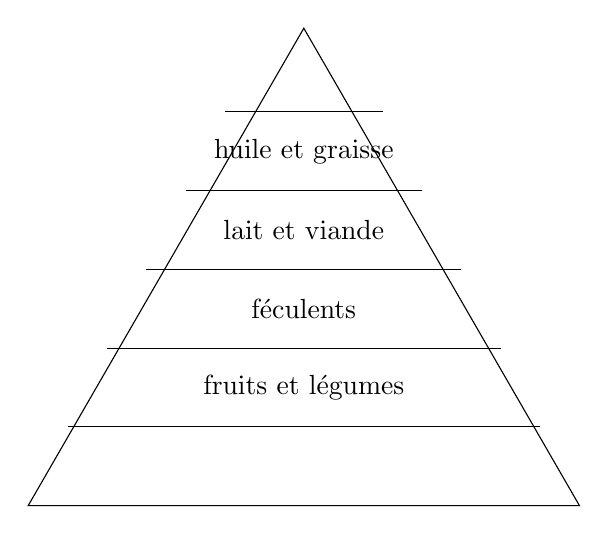
\begin{tikzpicture}
  \draw (0,0) -- (60:7) -- (7,0) -- cycle;
  \draw (0.5,1) -- (6.5,1);
  \draw (1,2) -- (6,2);
  \draw (1.5,3) -- (5.5,3);
  \draw (2,4) -- (5,4);
  \draw (2.5,5) -- (4.5,5);
  \node at (3.5,1.5) {fruits et légumes};
  \node at (3.5,2.5) {féculents};
  \node at (3.5,3.5) {lait et viande};
  \node at (3.5,4.5) {huile et graisse};
\end{tikzpicture}
\end{minipage}

\exercice{Le devenir des aliments}

\begin{minipage}[t][][t]{.4\linewidth}
  \question[]{Complétez les schéma du système digestif avec les légendes suivantes : \oe sophage, intestin grêle, bouche, anus, foie, gros intestin, estomac.}{7}{}{}

  \question{En quoi sont transformés les aliments dans le tube digestif ?}{1}{Ils sont transformés en nutriments}{\ligne{2}}

  \question{Donnez la définition de la digestion}{1}{C'est l'ensemble des tranformations chimiques et physiques qui transforment les aliments en nutriments.}{\ligne{6}}
\end{minipage}
\hfill
\begin{minipage}[t][][b]{.5\linewidth}
  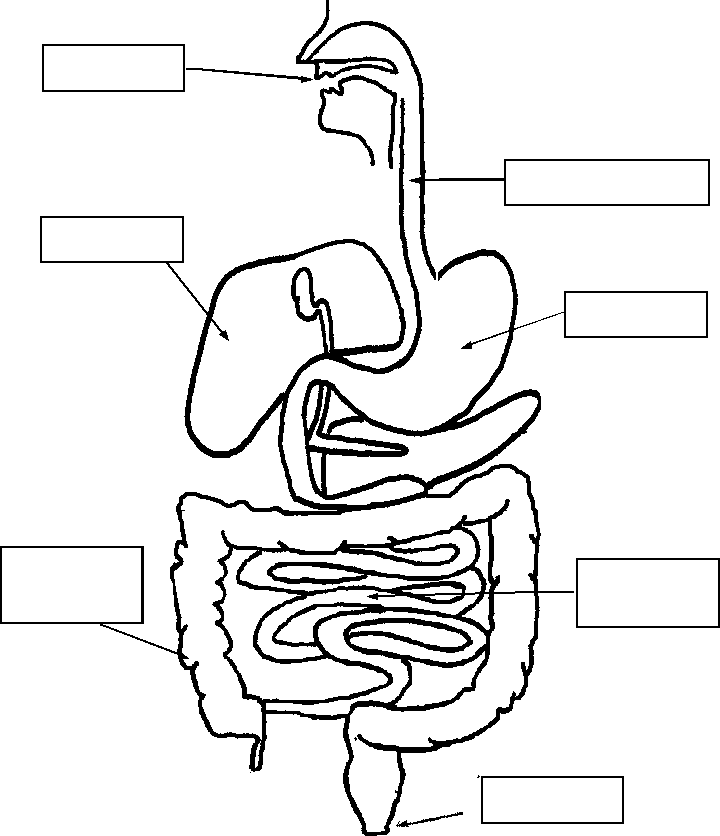
\includegraphics[width=9cm]{digestion.png}
\end{minipage}

\end{document}